\section{The Architecture} \label{The Architecture}

Initially we decided that we wanted to code our program in C\#\footnote{https://docs.microsoft.com/en-us/dotnet/csharp/getting-started/introduction-to-the-csharp-language-and-the-net-framework}. This was not an objective, analytical decision, but rather a sentimental question of preference and familiarity with the language. Our decision was also affected by the fact that C\# is a very popular language in the enterprise environment\cite{devstack}, which we also wanted to accommodate with the tool being general purpose.

Quite quickly it became evident that the machine learning frameworks available for C\# were lacklustre. There was a lack of documentation, which gave us issues with trying to set up the algorithms, and diversity, which gave us issues with testing the different approaches. We therefore decided to do machine learning with Python, since it has a rich, well-documented and diverse landscape of algorithms. This now meant we were building a C\#-program that will be utilizing Python. How we did this will be described later in section \ref{Python}.

\subsection{SOLID-principles} \label{SOLID-principles}

We wanted to keep our code in line with the SOLID-principles \cite{SOLID} as much as possible. The SOLID-principles are a set of guidelines that can help developers write better, cleaner and more maintainable code.
SOLID is an acronym of the following principles:
\begin{itemize}
    \item Single responsibility
    \item Open-Closed
    \item Liskov substitution
    \item Interface segregation
    \item Dependency inversion
\end{itemize}
These principles are described in the upcoming sections.

\subsection{Single Responsibility Principle}
This principle dictates that a class, module or function should be responsible for one single part of the functionality of a program. For example, if we want to load data, train a model and save the model (described in section \ref{Classifiers}), we need to write at least three functions. One for loading data, one for training the model, and one for saving the model. Of course, a function can be invoked by one of the others without violating the principle, but one function is not allowed to handle everything. This principle is sometimes also expressed as “A class should have only one reason to change”. \cite{SOLID}

\subsection{Open/Closed Principle}
This principle states that software should be open for extensions but should be closed for modification. This means that it should be possible to extend the behaviour of such an entity, without modifying its source code.

\subsection{Liskov Substitution Principle}
This principle extends upon the Open-closed principle, and adds the constraint that if a type S is a subtype of type T, then objects of type T can be replaced with objects of type S without changing the properties of the program. 
This means that everywhere the program expects some instance of T, we can use S instead, without the user noticing.
We use the Liskov substitution principle when predicting sentiment of different sentences. All our classifiers have the same interface and output, and therefore we can use the classifier specified by the user at runtime.

\subsection{Interface Segregation Principle}
This principle states that no client should be forced to depend on methods, that it does not use, and therefore it is better to create many small and specific interfaces, rather than larger ones. Following this principle helps lower coupling\footnote{In software engineering, coupling is the degree of interdependence between software modules; a measure of how closely connected two routines or modules are; the strength of the relationships between modules.} and therefore makes it easier to refactor or change the behaviour of the program. 

\subsection{Dependency Inversion Principle}
This principle states that it is better to depend on abstractions rather than concretions. Following this principle allows for easy switching between different modules implementing the same interface. We use this principle almost everywhere in the program. When we calculate the sentiment of a set of sentences, we use an implementation of the IEvaluator interface. This allowed us to implement multiple evaluators, and switch between them at runtime, rather than having to use the same one all the time.

\subsection{The Pipe}

We went with the pipe design pattern because this would enable us to create abstractions that easily adhered to the Liskov Substitution principle and the Single Responsibility principle. This allows us to run any evaluator with any given file using only one line of code, as shown below. This proved to be very useful, as switching between evaluators became very simple with this implementation. 
\begin{minted}{csharp}
	ThreadedSentenceLevelPipe(CSVReader.ReadCommentsYield, filename, evalr).ToList();
\end{minted}


The pipe pattern resembles the idea of an assembly line. For the programmer this means having clear, distinctive computations/stages that needs to be done in a sequence. The pattern is recognised to be especially effective when: \cite{pipeline}
\begin{itemize}
	\item The number of calculations is large compared to the number of stages. 
	\item It is possible to dedicate a processor to each element, or at least each stage, of the pipeline.
\end{itemize}
This fits our task that has clear stages that we need to put our data through: Load the data, pre-process it, evaluate it, analyse and output it again. The idea is also to create an abstraction that makes it easy for anyone to execute this sequence. In our case we implemented the pipe in such a way that we can easily swap a stage with another that does the same job e.g two different classifiers. 

Seen on figure \ref{pipe} is a diagram of how our pipe interacts with the program. For simplicity - importing and exporting has been omitted, but those of course is also a part of the process. 

\begin{figure}[H]
	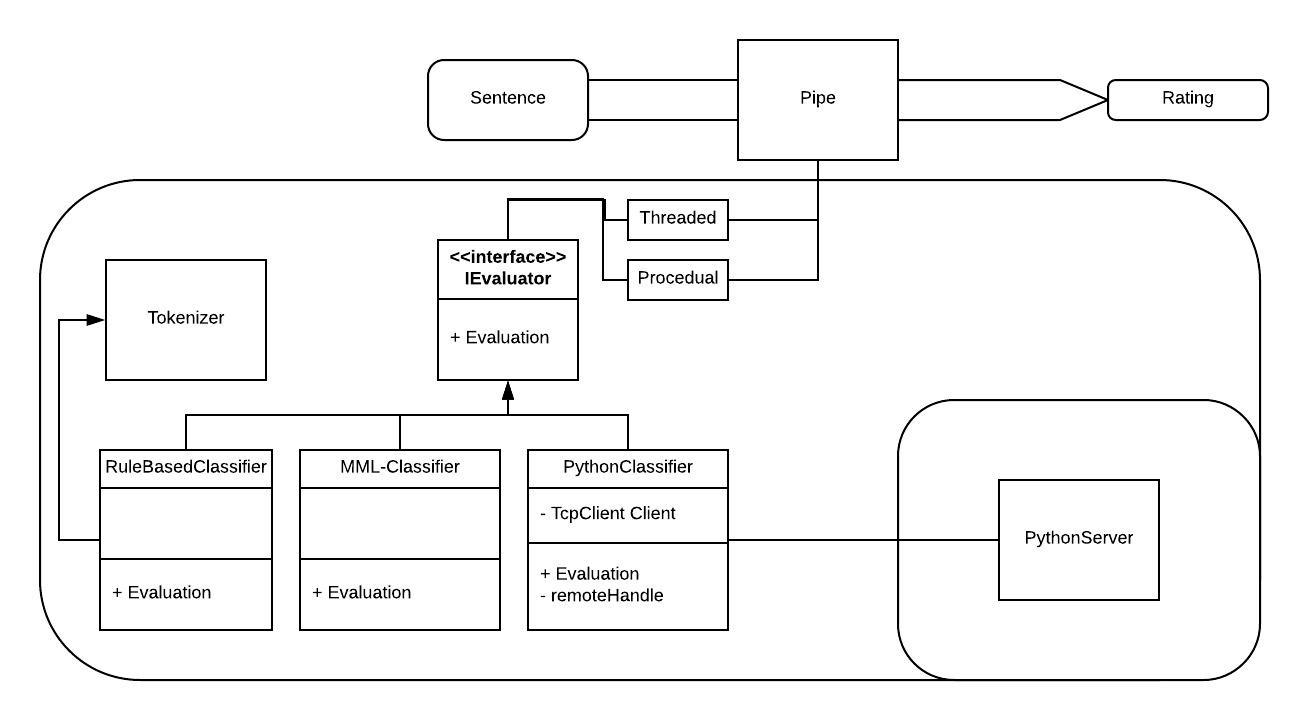
\includegraphics[width=\textwidth]{Images/Pipe}
	\centering
	\caption{UML Diagram of how the pipe works}
	\label{pipe}
\end{figure}

\subsection{Settings} \label{settings}

One of the goals of the program is to be general purpose. This also implies a level of customizability for the user, such that they can change the behaviour of the program to suit their needs. Most of the changes are limited to the Tokenizer, which is currently only used by our own rule based classifier. There are two different ways of altering the behaviour of the program: 
\begin{enumerate}
	\item By passing different arguments to the program at runtime
	\item Or by changing the settings within the settings.json-file.
\end{enumerate}
Not all our settings will be listed, but for the above two categories we have:

\begin{enumerate}
	\item Do predictions on input with the user specified classifier or take the input, shuffle it and return a document containing 10\% of the data and another with the rest. This is directly linked to training the different machine learning algorithms and testing them. 
	\begin{minted}{csharp}
		SAM svm -r /Data/MyDataToLabel.csv
		SAM data -r /Data/MyDataToSplit.csv
	\end{minted} 
	\item \begin{itemize}
		\item Multi Threaded or procedural - Please refer to Section \ref{parallelism} about parallelism.
		\item Expand abbreviations - Our rule based classifier can expand abbreviations, such that the lexicon will be able to match on the words. If the user wishes to parse a full comment to the program(multiple sentences), an abbreviation will inevitably make the program split a sentence at the punctuation, since the program can’t tell the difference between an abbreviation or the end of a sentence. Ultimately, this will not make a noticeable difference(if any) for the accuracy of our rule based classifier right now; however, since the tokenizer has this functionality, it may improve the accuracy of a future custom classifier as seen on figure \ref{abbrevexpand}.
		\item AbbreviationFinder Regex - The user is able to specify their own regular expression (regex) for finding abbreviations with the rule based classifier.
		\item Compare - The program can either label a dataset or load in a labelled dataset and determine the accuracy of the program.
		\item WriteNonMatchedTokens - This setting outputs a frequency list (in absolute numbers) of all the tokens that were not matched by the rule based classifier. This was a very useful tool when we we were expanding our lexicon.
	\end{itemize}
\end{enumerate}

\begin{figure}[H]
	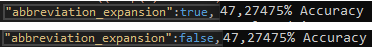
\includegraphics[width=\textwidth]{Images/AbbreviationCompare}
	\centering
	\caption{Comparison of Abbreviation Expansion}
	\label{abbrevexpand}
\end{figure}

\subsection{Python} \label{Python}
Initially we embedded Python in our C\#-program using an Adapter pattern. The adapter was created in such a way that it was interacting directly with a process that had a python terminal running with the Adapter pattern. \cite{adapter}
This very quickly ran into some unforeseen and very critical issues:
There was a character limit when passing arguments to the Python-terminal, which meant that we had to split up the sentences dynamically to fit within the length. This was mostly a nuisance, but still doable to program around. 
We could not keep the process running to continuously evaluate the arguments that we wanted to pass. We had to open a new process, load the model again and then rate the limited amount of comments mentioned above, which resulted in an unfeasible running time. We do not actually know how long it would have taken to rate all our sentences, because we stopped after 10 minutes and had only evaluated 378 sentences. Since we had 5500 sentences at the time of this experiment, it would have taken approximately two and a half hours to evaluate all sentences. 

Instead we created a Python server, which all our Python-related classifiers connect to when they want to do a request. This also now meant that in regards to the Open/Closed principle, anyone can easily add a different type of remote classifier that they want to interact with. It also satisfied the Liskov substitution principle, because the classifiers can be used interchangeably. This construct does have some limitations, which will be mentioned in the parallelism section.

For the classifiers themselves, the way we decided to build the python part of our program is very simple: Each classifier has its own script that handles training and evaluation (graphs and statistics) of the classifier, and then saves it using the dump function of the joblib package.
The neural network saved the model using a slightly different method, namely the built in saving function in Keras.
This essentially saves our trained classifier on disk with a small file size, allowing it to be loaded whenever needed. The idea behind this is threefold:
\begin{itemize}
	\item First and foremost, we do not have to train a classifier each time we want to use it. The only time we would want to do that is to change settings, or we have a new dataset.
	\item We can have multiple instances of the same classifier with different settings. 
	\item Lastly, we can close the program without losing our classifier - it will persist on the drive where the program is located.
\end{itemize}
The classifier is then saved with one of the the following filenames:
\begin{itemize}
	\item classifiername\_pipeline.joblib
	\item classifiername\_model.h5
\end{itemize}
As an example, the SVM will be saved as svm\_pipeline.joblib.
The reason it is called pipeline is because we use sklearns pipeline object. It allows us to create a list of transformers (like our TfidfVectorizer) and a final estimator (like our LinearSVC). Then we can call the transform and fit functions on the pipeline, just as we would on the individual transformers and estimators. Since it is not only the final estimator we wish to save, because the processing of the data is just as important, it allows us to save and load a single, compact file, instead of one for each transformer and the final estimator.

The saved file is used later in a script that handles phrases as input from the user. This script checks which classifier the user wishes to utilise for predicting the sentiment on a certain phrase (except if it’s the rule based classifier, this is handled by the C\# part of the program), and then loads the corresponding pipeline. Then the script gives the phrase to the pipeline that has been loaded in, which then predicts the sentiment of the phrase, and sends it back to the C\# part of the program, which finally hands it back to the user.


\subsection{Parallelism} \label{parallelism}
From the Pipe-pattern section it was noted that we have two different ways of running the pipe. One is doing it procedurally - handling one sentence at a time - and the other is a multi-threaded approach, which means handling multiple sentences at a time. In our program there are advantages and disadvantages to both approaches:

\begin{table}[H]
	\centering
	\begin{tabular}{@{}lllll@{}}
		\toprule
		& Procedural             & Multi-Threaded                  &  &  \\ \midrule
		Advantage    & Maintain order of data & Greatly decreased running time &  &  \\
		Disadvantage & Running time is slow   & Unordered data in output       &  &  \\
		&                        &                                 &  &  \\ \bottomrule
	\end{tabular}
	\caption{Parallelism Overview}
	\label{parallel}
\end{table}

On figure \ref{multiprog}, a running time comparison of the two is shown. This design decision reduced the running time of the program by 47\%. 

\begin{figure}[H]
	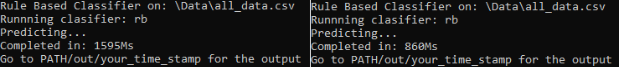
\includegraphics[width=\textwidth]{Images/MultithreadProgram}
	\centering
	\caption{Comparison of runtimes of the program.}
	\label{multiprog}
\end{figure}

The multi-threaded approach is currently limited to all of the classifiers that are part of the C\# program. Due to the difficulties of using Python together with C\# we chose to force procedural on python classifiers, because several factors made it unfavourable to make it so:
Firstly, it’s very resource demanding to do operations that talks in between programs or the operating system.
Running time itself increases when the program has to interact directly with the operating system. 
Secondly, it would be unavoidable to create a bottleneck and ultimately increase the running time drastically. This occurs because we’re running the python server locally. We can’t run many threads on the server because by limiting the thread supply and hence increasing the load on the CPU, we’re bottlenecking the C\#-program. Furthermore, we can’t run multiple threads in the C\#-program because the server then can’t handle all the incoming requests concurrently without being bottlenecked of same previous mentioned reason. Figure \ref{multiserv} shows how allowing a multithreaded approach currently will yield a far slower running time.
\begin{figure}[H]
	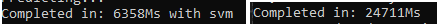
\includegraphics[width=\textwidth]{Images/MultithreadServer}
	\centering
	\caption{Comparison of runtimes of the server.}
	\label{multiserv}
\end{figure}

\subsection{Refresher}
In this section we introduced why we chose a C\# program that utilizes a Python server. We introduced the theory SOLID that affects our design decisions as well as some of the settings that are available to a user. Lastly we introduced our pipe-pattern together with our parallelism.
